%% LaTeX Beamer presentation template (requires beamer package)
%% see http://bitbucket.org/rivanvx/beamer/wiki/Home
%% idea contributed by H. Turgut Uyar
%% template based on a template by Till Tantau
%% this template is still evolving - it might differ in future releases!

\documentclass{beamer}
\mode<presentation>
{
% 	\usetheme{Singapore}
	\usetheme{Dresden}
	\setbeamertemplate{footline}[frame number]
	\usefonttheme{serif}

	\setbeamertemplate{navigation symbols}{}
    \setbeamertemplate{caption}[numbered]
% 	\setbeamercovered{transparent}
}

\usepackage{cancel}
\usepackage{amsmath}
\usepackage{graphics}

\usepackage{ulem}
\normalem

\usepackage{wasysym}

\usepackage{mdframed}

\usepackage{algorithm}
\usepackage[noend]{algpseudocode}

\usepackage{multicol}

\title{Graph Decomposition (2)}
\subtitle{--- BFS and its Applications}

\author{Hengfeng Wei}
\institute{hengxin0912@gmail.com}

\date{\today}

% Delete this, if you do not want the table of contents to pop up at
% the beginning of each subsection:
\AtBeginSubsection[]
{
	\begin{frame}<beamer>
		\frametitle{Outline}
		\tableofcontents[currentsection]
	\end{frame}
}

\AtBeginSection[]
{
	\begin{frame}<beamer>
		\frametitle{Outline}
		\tableofcontents[currentsection]
	\end{frame}
}
% If you wish to uncover everything in a step-wise fashion, uncomment
% the following command:

%\beamerdefaultoverlayspecification{<+->}

\begin{document}

\begin{frame}
	\titlepage
\end{frame}

\begin{frame}
	\frametitle{Outline}
	\tableofcontents
% You might wish to add the option [pausesections]
\end{frame}

%%%%%%%%%%%%%%%%%%%
\section{BFS: Algorithm}

\begin{frame}{Problem}
  \begin{exampleblock}{Problem: Shortest Path}
    Given an undirected graph $G = (V, E)$ and a source vertex $s$,
    to compute distance $\delta(s, u)$ for each vertex $u$.
  \end{exampleblock}

  \[
    \delta(s,u) \equiv \# \textrm{ of edges of the shortest path between } s
    \textrm{ and } u.
  \]
\end{frame}
%%%%%%%%%%%%%
\begin{frame}{BFS on Undirected Graph}
  BFS with source vertex $s$:
  \begin{itemize}
    \item exploring every vertex $u$ reachable from $s$
    \item \textcolor{purple}{computing $\delta(s,u)$, for all reachable $u$}
  \end{itemize}

  \vspace{0.50cm}
  BFS as a framework:
  \begin{itemize}
    \item Prim's MST algorithm
    \item Dijkstra's SSSP algorithm
  \end{itemize}
\end{frame}
%%%%%%%%%%%%%
\begin{frame}{A Physical Algorithm of BFS (\textsf{Phys-BFS})}
  \begin{columns}
    \column{0.50\textwidth}
	  \begin{figure}[htp]
	    \centering
		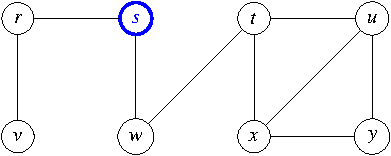
\includegraphics[width = 0.85\textwidth]{figure/bfs-graph.pdf}
	  \end{figure}
    \column{0.50\textwidth}
	  \begin{figure}[htp]
	    \centering
		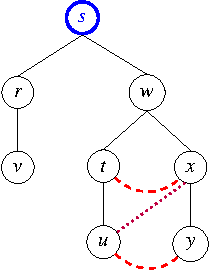
\includegraphics[width = 0.50\textwidth]{figure/bfs-physical-alg.pdf}
	  \end{figure}
  \end{columns}
\end{frame}
%%%%%%%%%%%%%
\begin{frame}{Edge Properties of \textsf{Phys-BFS}}
  \begin{mdframed}[linecolor = blue, leftmargin = 2cm, rightmargin = 2cm]
    \[ (u,v) \in E \Rightarrow d(u) \le d(v) \le d(u) + 1 \]
  \end{mdframed}
\end{frame}
%%%%%%%%%%%%%
\begin{frame}{A Parallel Algorithm of BFS (\texttt{Para-BFS})}
  \begin{description}
    \item[graph:] network of computers
    \item[vertex:] computer
    \item[edge:] network connections
  \end{description}

  \vspace{0.50cm}
  \begin{center}
  	To disseminate a computer virus from computer $s$.
  \end{center}
\end{frame}
%%%%%%%%%%%%%
\begin{frame}{Color Properties in \texttt{Para-BFS}}
  \begin{displaymath}
	\textrm{states of computers} = \left\{ \begin{array}{ll}
	\texttt{WHITE} & \textrm{if healthy}\\
	\texttt{GRAY} & \textrm{if infected}
	\end{array} \right.
  \end{displaymath}
\end{frame}
%%%%%%%%%%%%%
\begin{frame}{A Parallel Algorithm of BFS (\texttt{Para-BFS})}
  \begin{algorithm}[H]
    \caption{A Parallel Algorithm of BFS (\texttt{Para-BFS}).}
    \begin{multicols}{2}[\columnsep = -50pt]
    \begin{algorithmic}[]
    {\footnotesize
      \Procedure{Para-BFS}{$G, s$}
		\ForAll{$u \in V$}
		  \State color[$u$] $\gets$ \texttt{WHITE}
		  \State d[$u$] $\gets$ $\infty$
		\EndFor

		\Statex
		\State color[$s$] $\gets$ \texttt{GRAY}
		\State d[$s$] $\gets$ $\infty$

		\Statex
		\State \textcolor{purple}{\textrm{Q} $\gets$ $\{ s \}$}
		\While{\textrm{Q} $\neq$ $\emptyset$}
		    \State \textcolor{purple}{$u$ $\gets$ Deq(\textrm{Q})}
			\ForAll{$(u,v) \in E$}
			  \If{color[$v$] = \texttt{WHITE}}
			    \State \textcolor{blue}{color[$v$] = \texttt{GRAY}}
			    \State d[$v$] = d[$u$] + 1
			    \State \textcolor{purple}{Enq(\textrm{Q}, $v$)}
			  \EndIf
			\EndFor
			\State \textcolor{blue}{color[$u$] $\gets$ \texttt{BLACK}}
		  \EndFor
		\EndWhile
      \EndProcedure
    }
    \end{algorithmic}
    \end{multicols}
  \end{algorithm}
\end{frame}
%%%%%%%%%%%%%
\begin{frame}{Color Properties of \texttt{Para-BFS}}
  States of vertices:
  \begin{description}
    \item [\texttt{WHILE:}] undiscovered
    \item [\texttt{GRAY:}]	discorvered but
    \item [\texttt{BLACK:}]	discorvered and all its neighbors has been
    discorvered
  \end{description}

  \begin{center}
  	\texttt{WHITE} $\Rightarrow$ \texttt{GRAY} $\Rightarrow$ \texttt{BLACK}
  \end{center}

  \begin{enumerate}
    \item $(u,v) \in E$, $u$ is \texttt{BLACK} $\Rightarrow$ $v$ is either
    \texttt{BLACK} or \texttt{GRAY}
    \item \texttt{GRAY} vertex may have adjacent \texttt{WHITE} vertices
    \\ $\Rightarrow$ ``frontier'' between discovered and undiscovered vertices
    \item Invariant: at any time, all \texttt{GRAY} vertices are in the Queue
  \end{enumerate}
\end{frame}
%%%%%%%%%%%%%
\begin{frame}{Correctness Proof \texttt{Para-BFS}}

\end{frame}
%%%%%%%%%%%%%
\begin{frame}{BFS Algorithm}

\end{frame}
%%%%%%%%%%%%%%%%%%%
\section{BFS: Properties}

%%%%%%%%%%%%%
\begin{frame}{Color Properties}

\end{frame}
%%%%%%%%%%%%%
\begin{frame}{Queue Properties}

\end{frame}
%%%%%%%%%%%%%
\begin{frame}{Correctness Proof}

\end{frame}
%%%%%%%%%%%%%
\begin{frame}{Edges Properties}

\end{frame}
% %%%%%%%%%%%%%%%%%
\section{BFS: Applications}

%%%%%%%%%%%%%
\begin{frame}{Testing Bipartiteness}

\end{frame}
%%%%%%%%%%%%%
\begin{frame}{}

\end{frame}
%%%%%%%%%%%%%
\begin{frame}{}

\end{frame}
%%%%%%%%%%%%%%%%%%
\section*{Summary}
\begin{frame}{}
  \begin{figure}[htp]
    \begin{center}
      
\includegraphics[width=0.618\textwidth]{figure/thankyou.jpg}
    \end{center}
  \end{figure}
\end{frame}
%%%%%%%%%%
\end{document}
